\documentclass[10pt]{article}
\usepackage[T1]{fontenc}
\usepackage[margin=0.62in]{geometry}
\usepackage{array}
\usepackage{tikz}
\usetikzlibrary{arrows.meta,positioning,calc}

\pagestyle{plain}
\setlength{\parindent}{0pt}
\setlength{\parskip}{0.28em}
\emergencystretch=3em
\renewcommand{\arraystretch}{1.08}

\newcolumntype{L}[1]{>{\raggedright\arraybackslash}p{#1}}
\tikzset{
  box/.style={draw, rounded corners=1pt, align=center, inner sep=4pt, minimum height=8mm},
  smallbox/.style={draw, rounded corners=1pt, align=center, inner sep=3pt, font=\scriptsize},
  edge/.style={-{Stealth[length=2mm]}, thick},
  faintedge/.style={-{Stealth[length=2mm]}, thick, dashed}
}

\begin{document}

\begin{center}
{\Large Uncut Gem NV Diamond Magnetometer}\\
{\normalsize Dense build-state, board-flow, and fixed-board model}\\
worlds session, 2026-06-02
\end{center}

\section*{Verdict}

\begin{center}\small
\begin{tabular}{|L{1.1in}|L{4.3in}|L{0.65in}|}
\hline
\textbf{Plane} & \textbf{Dense status} & \textbf{Gate} \\
\hline
Identity & Quantum Village Uncut Gem: NV-center diamond magnetometer, not EEG,
fNIRS, or BCI. Signal is ODMR fluorescence near 2.87 GHz. & fixed \\
\hline
Local build & One KiCad PCB plus optional INA333 acquisition-isolation branch.
Stock includes MMG3014NT1, headers, photodiode sockets, photodiodes. & partial \\
\hline
Open blockers & Stocked vertical SMA does not fit Molex edge footprint; RF amp
population must be inspected; optical geometry and detector baseline remain
unproven. & hold \\
\hline
Success claim & A valid build requires rails, ESP32 boot, PLL lock, RF continuity,
aligned laser/diamond/antenna, detector baseline, and repeatable ODMR trace. & proof \\
\hline
\end{tabular}
\end{center}

\section{Whole-device flow}

\begin{center}
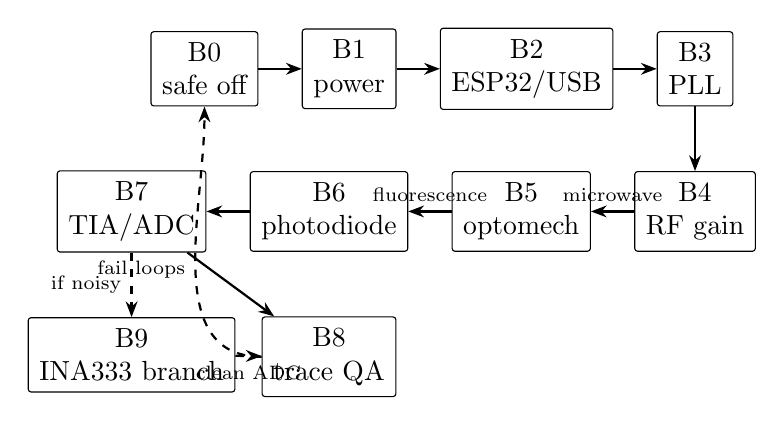
\begin{tikzpicture}[node distance=0.82cm and 0.55cm]
\node[box] (safe) {B0\\safe off};
\node[box, right=of safe] (pwr) {B1\\power};
\node[box, right=of pwr] (esp) {B2\\ESP32/USB};
\node[box, right=of esp] (pll) {B3\\PLL};
\node[box, below=of pll] (rf) {B4\\RF gain};
\node[box, left=of rf] (opt) {B5\\optomech};
\node[box, left=of opt] (pd) {B6\\photodiode};
\node[box, left=of pd] (tia) {B7\\TIA/ADC};
\node[box, below=of pd] (qa) {B8\\trace QA};
\node[box, below=of tia] (ina) {B9\\INA333 branch};

\draw[edge] (safe) -- (pwr);
\draw[edge] (pwr) -- (esp);
\draw[edge] (esp) -- (pll);
\draw[edge] (pll) -- (rf);
\draw[edge] (rf) -- node[above, font=\scriptsize]{microwave} (opt);
\draw[edge] (opt) -- node[above, font=\scriptsize]{fluorescence} (pd);
\draw[edge] (pd) -- (tia);
\draw[edge] (tia) -- (qa);
\draw[faintedge] (tia) -- node[left, font=\scriptsize]{if noisy} (ina);
\draw[faintedge] (ina) -- node[below, font=\scriptsize]{clean ADC} (qa);
\draw[faintedge] (qa.west) to[out=180,in=270] node[left, font=\scriptsize]{fail loops} (safe.south);
\end{tikzpicture}
\end{center}

\section{Actual board-state matrix}

\begin{center}\scriptsize
\begin{tabular}{|L{0.35in}|L{0.9in}|L{1.75in}|L{1.65in}|L{1.35in}|}
\hline
\textbf{S} & \textbf{Where} & \textbf{What / how} & \textbf{Why} & \textbf{Exit proof} \\
\hline
B0 & safety & Laser/RF off; exposed 5 V untrusted. & Prevent eye/RF/electrical damage before proof. & No powered emission. \\
\hline
B1 & P1, 5V, U6 & USB-C or 5V\_SUPP feeds protection and LM1117 3.3 V. & Logic and RF tests depend on stable rails. & 5 V and 3.3 V measured. \\
\hline
B2 & U8, U7, OLED & CP2102N programs ESP32; BOOT/EN select flash/run; OLED and serial report state. & Firmware is the coordinator for PLL, laser, ADC. & Boot log plus OLED alive. \\
\hline
B3 & X1, U1, SPI & 10 MHz clock drives ADF4351; ESP32 writes SPI registers and checks lock/output. & No ODMR sweep without coherent microwave source. & PLL lock or known RF output. \\
\hline
B4 & J1, U2/U3, J4 & Correct edge SMA only; inspect MMG3014NT1 amps, bias, matching, DNP RF outputs. & RF faults must be isolated from optics/acquisition. & Fit, continuity, bias sane. \\
\hline
B5 & laser, diamond, antenna & Co-locate 520 nm laser spot, NV diamond, microwave antenna, printed holder. & Resonance changes fluorescence only at the shared geometry. & Visible alignment. \\
\hline
B6 & PHOTODIODE1, D4 & Socket or BPW34-equivalent DNP footprint converts red fluorescence to current. & This is the physical measurement boundary. & Dark/light contrast. \\
\hline
B7 & U5, J6, TP1/TP2 & TL082 conditions detector current; ADC\_SIGNAL reaches ESP32 and debug probes. & Trace quality is decided before firmware plotting. & Unsaturated baseline. \\
\hline
B8 & sweep QA & ESP32 sweeps 128 points, averages ADC, and streams the trace. & Only here can an ODMR dip be claimed. & Repeatable dip. \\
\hline
B9 & INA333 daughterboard & Optional reversible isolation: detector-side input to INA333, one clean ADC driver. & Fixes coupled RF/detector noise without redesigning PCB. & Lower noise, no RF regression. \\
\hline
\end{tabular}
\end{center}

\section{Counterfactual fixed board}

\begin{center}
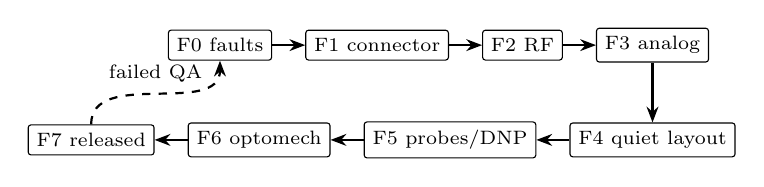
\begin{tikzpicture}[node distance=0.76cm and 0.42cm]
\node[smallbox] (f0) {F0 faults};
\node[smallbox, right=of f0] (f1) {F1 connector};
\node[smallbox, right=of f1] (f2) {F2 RF};
\node[smallbox, right=of f2] (f3) {F3 analog};
\node[smallbox, below=of f3] (f4) {F4 quiet layout};
\node[smallbox, left=of f4] (f5) {F5 probes/DNP};
\node[smallbox, left=of f5] (f6) {F6 optomech};
\node[smallbox, left=of f6] (f7) {F7 released};
\draw[edge] (f0) -- (f1);
\draw[edge] (f1) -- (f2);
\draw[edge] (f2) -- (f3);
\draw[edge] (f3) -- (f4);
\draw[edge] (f4) -- (f5);
\draw[edge] (f5) -- (f6);
\draw[edge] (f6) -- (f7);
\draw[faintedge] (f7.north) to[out=90,in=270] node[above, font=\scriptsize]{failed QA} (f0.south);
\end{tikzpicture}
\end{center}

\begin{center}\scriptsize
\begin{tabular}{|L{0.35in}|L{1.0in}|L{2.45in}|L{2.1in}|}
\hline
\textbf{F} & \textbf{Fix plane} & \textbf{Counterfactual board change} & \textbf{Dense criterion} \\
\hline
F0 & observed faults & Wrong SMA inventory, unproven RF amps, noisy/ambiguous acquisition path. & Target remains grounded in actual failures. \\
\hline
F1 & connector & PCB footprints match intended RF connector family and edge constraints. & No "force the SMA" branch. \\
\hline
F2 & RF topology & U2/U3, bias, matching, DNP outputs, and gates are one documented microwave path. & RF faults become directly diagnosable. \\
\hline
F3 & analog front end & INA333-style isolation or redesigned TL082 path is native to schematic/layout. & One quiet owner of ADC\_SIGNAL. \\
\hline
F4 & layout partition & RF current, laser switching, analog return, and detector input are separated/guarded. & Less fake fluorescence from coupling. \\
\hline
F5 & debug contract & J6, TP1, TP2/MUX\_OUT, RF DNP points named in silkscreen, BOM, test plan. & Debug surfaces are not guesses. \\
\hline
F6 & geometry & Laser, diamond, antenna, photodiode constraints tied to STL/STEP/fiducials. & ODMR depends on geometry, not only continuity. \\
\hline
F7 & release & Main PCB reaches B8 without B9: rails, PLL, RF, optics, detector, trace all pass. & Fixed board makes the daughterboard unnecessary. \\
\hline
\end{tabular}
\end{center}

\section{BOM and build gates}

\begin{center}\scriptsize
\begin{tabular}{|L{1.15in}|L{1.45in}|L{3.25in}|}
\hline
\textbf{Area} & \textbf{Stock / evidence} & \textbf{Action gate} \\
\hline
Power/USB & USB-C, 2x3 headers & Verify P1/5V\_SUPP polarity, protection, U6 output before downstream load. \\
\hline
Controller & ESP32, CP2102N, OLED header & Flash firmware; prove serial/OLED before RF emission. \\
\hline
PLL/RF & ADF4351, X1, MMG3014NT1 x8 & Inspect population; verify bias/matching; reject wrong vertical SMA for J1. \\
\hline
Optics & STL/STEP, laser, diamond, antenna & Align laser spot, antenna, diamond, detector before interpreting trace. \\
\hline
Detector & MTCELL socket, photodiode x5 & Confirm BPW34-equivalent orientation and socket/D4 path. \\
\hline
Rework & INA333 stock, headers/probes & Map U5/J6/TP nodes; isolate old output before any clean ADC injection. \\
\hline
\end{tabular}
\end{center}

\section{Proof checklist}

\begin{center}\scriptsize
\begin{tabular}{|L{1.25in}|L{2.2in}|L{2.25in}|}
\hline
\textbf{Claim} & \textbf{Evidence required} & \textbf{Rollback if missing} \\
\hline
Buildable & Rail measurements, boot log, J1-compatible connector, U2/U3 inspection. & Return to B0/B1/B4. \\
\hline
Microwave source & PLL register trace, lock/output proof, RF continuity/bias. & Return to B3/B4. \\
\hline
Optical coupling & Laser/diamond/antenna/detector photo and dark/light detector contrast. & Return to B5/B6. \\
\hline
ODMR candidate & Repeatable sweep with baseline, dip, and same settings recorded. & Return to B7/B8. \\
\hline
INA333 improvement & Stock-vs-rework noise comparison plus unchanged RF sweep. & Revert B9. \\
\hline
\end{tabular}
\end{center}

\section{Evidence and artifacts}

\begin{itemize}
\item \texttt{p/place/trees/bcf-0031.tree}: canonical Uncut Gem NV magnetometer tree.
\item \texttt{p/place/trees/bcf-0036.tree}: JLCPCB and gerber audit context.
\item \texttt{p/place/trees/scan-0087.tree}: local STL/station context.
\item \texttt{p/place/bci/devices/uncut-gems-build.tree}: transcludable dense model.
\item \texttt{p/place/build/latex/uncut-gems/uncut-gems-state-machine.pdf}: this rendered artifact.
\item Upstream \texttt{QuantumVillage/UncutGem}: firmware, KiCad, STEP/STL.
\end{itemize}

\textbf{Safety.} Laser and RF instrument. No BCI claim. Verify eye safety, RF handling,
5 V integrity, connector fit, thermal behavior, and trace repeatability before operation.

\end{document}
